\chapter{The Standard Model}

\textit{"...it turns out that based on their findings, which will be confirmed
or contradicted when the Swiss machine is up and running, turns out there's
slightly more positive than negative muons in all of our atoms, which would
justify the faith of all the believers of the world, make you more
optimistic, and give us an explanation for how we might have all come to this
moment from the primordial slime."}
\vspace{5mm}
\begin{flushright}
--- Bill Clinton, Davos 2011
\end{flushright}

\thispagestyle{empty}
\newpage

\noindent
Our current best understanding of Nature is that the dynamics of matter is governed
by four fundamental forces. General Relativity (GR) provides a
description of spacetime, the arena in which matter exists and interacts, and asserts
that spacetime is not a static entity but is rather dynamically shaped by the presence
of matter and energy. It also explains one of the forces, the gravitational force, as an apparent
phenomenon arising from geodesic motion in curved spacetime. The Standard Model of particle physics
(SM) not only describes the remaining three forces, the electromagnetic (EM) force,
the weak force, and the strong force, but also provides a description of matter, and 
elucidates the origin of mass.

The Standard Model is expressed in the language of Quantum Field Theory (QFT). QFT 
extends the domain of quantum mechanics, which characterises the very small, to
the domain of special relativity, which governs the very fast. It does so by
proposing that the fundamental objects are not particles, but rather fields, the
excitations of which are interpreted as particles.

Similarly to classical field theory the system under consideration is fully characterised
by a Lagrangian density, usually simply called the Lagrangian. According to
the principle of least action, the equations of motion for a system are then derived
by solving the Euler-Lagrange equation,
\begin{equation}
\partial_\mu \left(\frac{\partial \mathcal{L}}{\partial(\partial_\mu \phi_i)}\right)
- \frac{\partial{\mathcal{L}}}{\partial \phi_i} = 0,
\end{equation}
where $\mathcal{L}$ is the Lagrangian, $\phi_i$ are the fields, whose explicit dependence
on $x^\mu$ is suppressed for clarity, partial derivatives
are taken with respect to the spacetime coordinates, and Einstein summation convention implies
the sum over repeated indices \cite{Thomson:2013zua}. The Lagrangian therefore contains all
information about the dynamical system. 

The Lagrangian must be invariant under the transformations which leave the
system it describes physically unchanged. Apart from the Poincar\'e symmetries, which
ensure the physics is invariant w.r.t. translations, rotations, and changes of inertial
reference frame, the defining symmetry of the Standard Model is the internal
$\text{SU}(3)_C \times \text{SU}(2)_L \times \text{U}(1)_Y$ local gauge redundancy.

The $\text{SU}(3)_C$ group symmetry, where $C$ stands for colour, defines quantum chromodynamics
(QCD), the theory of strong force interactions between quarks and gluons. The electroweak
interactions, a unified theory of the electromagnetic and weak forces, are described by
the $\text{SU}(2)_L \times \text{U}(1)_Y$ group symmetry. Here, the $L$ refers to left-handed
chirality, which is related to the relative direction of the particle momentum and spin, and
$Y$ is the weak hypercharge \cite{Thomson:2013zua} explained later in this chapter.

The requirement for the Lagrangian to be locally gauge-invariant places some constraints
on the allowed terms. Notably, the four-derivative $\partial_\mu$ is replaced by a 
covariant derivative, which introduces the interactions between the matter and gauge
fields. On the other hand, local gauge invariance prohibits the naive mass terms for
both the gauge bosons and fermions \cite{Thomson:2013zua}. This is in stark contrast
with experimental reality: fermions and weak gauge bosons are massive.

This embarrassing discrepancy is resolved by the Higgs mechanism, which generates the
masses of the fermions and gauge bosons by interactions with the non-zero Higgs field
value at the minimum of the Higgs potential.

\section{Elementary particles}

The particle content of the Standard Model can be classified according to spin, the
intrinsic angular momentum. Particles with half-integer spin obey Fermi-Dirac statistics
and are called fermions, while particles with integer spin obey Bose-Einstein
statistics and are called bosons.

\begin{table}[h]
\centering
\caption{Fermions of the Standard Model}
\label{tab:the:fermions}
\begin{tabular}{c c ccc ccc}
\toprule
\midrule
 & & \multicolumn{3}{c}{generation} & \multicolumn{3}{c}{interaction} \\ 
 & & \nth{1} & \nth{2} & \nth{3} & weak & EM & strong \\
\midrule
\multirow{2}{*}{\textbf{Quarks}}
& up-type    & $u$ & $c$ & $t$ & \cmark & \cmark & \cmark \\
& down-type  & ~$d$~ & ~$s$~ & ~$b$~ & \cmark & \cmark & \cmark \\
\multirow{2}{*}{\textbf{Leptons}}
& charged    & ~$e$~ & ~$\mu$~ & ~$\tau$~ & \cmark & \cmark & \\
& neutrinos  & ~$\nu_e$~ & ~$\nu_\mu$~ & ~$\nu_\tau$~ & \cmark & & \\
\midrule
\bottomrule
\end{tabular}
\end{table}

All known fundamental (i.e. non-composite) fermions have spin-$\frac{1}{2}$ and are
shown in Table \ref{tab:the:fermions}. They are categorised as quarks, which interact via
the strong force, and leptons, which don't. Both quarks and charged leptons interact
via the electromagnetic force, and all fermions interact via the weak force.
Both quarks and leptons exist in six flavours, i.e. distinct species, and come in
generations. In the Standard Model, there
are three generations of up- and down-type quarks as well as charged leptons and
neutrinos. The electromagnetic charges of up-type quarks are $+2/3 e$, those of down-type
quarks are $-1/3 e$, and those of charged leptons are $-1 e$, where $e$ is the magnitude of
the charge of the electron. The masses of quarks and charged leptons increase with
each generation, while the pattern is presently unknown for neutrinos.

\begin{table}[h]
\centering
\caption{Bosons of the Standard Model}
\label{tab:the:bosons}
\begin{tabular}{c c ccc}
\toprule
\midrule
 & & & multiplicity & interaction \\ 
\midrule
\multirow{4}{*}{\textbf{Spin-1}}
 & photon    & $\gamma$ & 1 & EM      \\
 & $Z$ boson & $Z$      & 1 & weak    \\
 & $W$ boson & $W^\pm$  & 2 & weak    \\
 & gluon     & $g$      & 8 & strong  \\
\textbf{Spin-0} & Higgs boson & $H$ & 1 &  \\
\midrule
\bottomrule
\end{tabular}
\end{table}

Vector (spin-1) bosons in the Standard Model are the force carriers, the photon for the
electromagnetic interaction, the $Z$ and $W$ bosons for the weak interaction,
and the gluons for the strong interaction. Photons and gluons are massless, but
the $Z$ and $W$ bosons are among of the heaviest fundamental particles in the
Standard Model. The $W$ boson comes in two variants, $W^+$ is positively charged
and $W^-$ negatively charged. Gluons come in eight variants, each with a unique
colour charge combination. The Higgs boson is the only known fundamental scalar
(spin-0) \cite{Thomson:2013zua}.

Neutrons and protons are examples of hadrons, composite particles made of quarks
and gluons, collectively known as partons. The proton consists of two $u$ and one
$d$ valence quarks, in addition to the sea of virtual gluons giving rise to an
antiquark component through gluon splitting to quark-antiquark pairs. Partons
each carry a fraction of the proton momentum, characterised by the Bjorken $x$
variable. The interactions between the proton constituents results in a
distribution of parton momenta within the proton, which is parametrised by the
parton distribution functions (PDFs).

\section{Electroweak interactions}

Quantum electrodynamics (QED) describes the interaction between charged fermions
mediated by the photon. In order for the Lagrangian to be invariant
under local $\text{U}(1)$ transformation of the fermion fields,
\begin{equation}
\psi(x) \rightarrow \psi'(x) = e^{iq\chi(x)}\psi(x),
\end{equation}
where $\psi$ is a fermion field, $q$ is the charge, and $\chi(x)$ is local choice of
the gauge, the four-derivative in the naive Dirac Lagrangian must be replaced by
the covariant derivative,
\begin{equation}
\partial_\mu \rightarrow D_\mu = \partial_\mu + i q A_\mu,
\end{equation}
where $A_\mu$ is the photon gauge field which transforms as
\begin{equation}
A_\mu \rightarrow A_\mu' = A_\mu - \partial_\mu \chi(x)
\end{equation}
\cite{Thomson:2013zua}.
%This results in the following Lagrangian term for
%QED interactions between a fermion of mass $m$ and charge $q$ and the massless photon $A_\mu$:
%\begin{equation}
%\mathcal{L}_{\text{QED}} =
%i\bar{\psi}\gamma^\mu D_\mu \psi - m\bar\psi\psi - \frac{1}{4}F_{\mu\nu}F^{\mu\nu},
%\end{equation}
%where $\gamma^\mu$ is the gamma matrix and $F_{\mu\nu} = \partial_\mu A_\nu - \partial_\nu A_\mu$
%is the field strength tensor.

Similarly, the weak interaction is related to the invariance under $\text{SU}(2)_L$ local
phase transformation of left-handed weak isospin doublets:
\begin{equation}
\varphi(x) = \begin{pmatrix} \nu_e(x) \\ e(x) \end{pmatrix} \rightarrow
\varphi' = (\mathbf{I} + i g_W \mathbf{\alpha}(x)\cdot\mathbf{T}) \varphi(x),
\end{equation}
where $\mathbf{I}$ is the $2\times2$ identity matrix, $g_W$ is the weak coupling constant,
$\alpha(x)$ are the three local choices of gauge, and $\mathbf{T} = \frac{1}{2}\sigma$,
where $\sigma$ are the Pauli spin-matrices, are the three generators of the $\text{SU}(2)$ group.
In order to achieve the gauge invariance of the Lagrangian under $\text{SU}(2)$ the four-derivative
is replaced by the covariant derivative,
\begin{equation}
\partial_\mu \rightarrow D_\mu = \partial_\mu + i g_W \mathbf{T} \cdot \mathbf{W}_\mu(x),
\end{equation}
where $\mathbf{W}_\mu(x)$ are the gauge fields of the weak interaction \cite{Thomson:2013zua}.

A unified theory of quantum electrodynamics (QED) and the weak interaction was developed
by Glashow, Salam, and Weinberg (GSW) in the 1960s \cite{Thomson:2013zua} to make the
theory compatible with the fact that the observed $Z$ boson couples to both left- and
right-handed particles. To this end, a new $\text{U}(1)_Y$ symmetry is introduced with a new gauge
field $B_\mu$, coupling $g'$, and a new charge $Y$, called the weak hypercharge. In this unified model,
the physical bosons are the mixtures of the gauge fields
\begin{equation}
A_\mu = B_\mu \cos\theta_W + W_\mu^{(3)} \sin{\theta_W},
\end{equation}
\begin{equation}
Z_\mu = - B_\mu \sin{\theta_W} + W_\mu^{(3)} \cos{\theta_W},
\end{equation}
\begin{equation}
W^+_\mu = \frac{1}{\sqrt{2}}\left( W_\mu^{(1)} - W_\mu^{(2)} \right),
\end{equation}
\begin{equation}
W^-_\mu = \frac{1}{\sqrt{2}}\left( W_\mu^{(1)} + W_\mu^{(2)} \right),
\end{equation}
and the couplings to the photon and $W$ are related as $e = g_W \sin{\theta_W}$,
while the coupling to the $Z$ boson turns out to be $g_Z  = \frac{g_W}{\cos{\theta_W}}$.
The weak hypercharge $Y$ is related to the elecric charge and the third component of weak
isospin as $Y = 2(Q - I_W^{(3)})$ \cite{Thomson:2013zua}.

In this $\text{SU}(2)_L \times \text{U}(1)_Y$ model, however, the naive mass terms of the form $-m\bar\psi\psi$
are no longer gauge-invariant and thus both the fermions and the bosons are massless in this theory.
To reconcile this with the experimental reality of massive fermions and $W$ and $Z$ bosons, a
mechanism is needed which would result in gauge-invariant mass terms \cite{Thomson:2013zua}.

\section{The Higgs mechanism}

The simplest Higgs model is a weak isospin doublet of complex scalar fields \cite{Thomson:2013zua},
\begin{equation}
\phi = \begin{pmatrix} \phi^+ \\ \phi^0 \end{pmatrix},
\end{equation}
described by the Lagrangian
\begin{equation}
\mathcal{L} = (\partial_\mu \phi)^\dag (\partial^\mu \phi) - \mu^2(\phi^\dag\phi) - \lambda(\phi^\dag \phi)^2,
\label{eq:higgs_lag}
\end{equation}
where the potential $V(x) = \mu^2(\phi^\dag\phi) + \lambda(\phi^\dag \phi)^2$
has an infinite number of minima satisfying $\phi^\dag \phi = -\frac{\mu^2}{2\lambda}$
in the case when $\mu^2 < 0$ \cite{Thomson:2013zua}. The symmetry is spontaneously broken by choosing a
particular minimum from the allowed set, and the fields can be expanded around the chosen minimum.
In the unitary gauge, the Higgs doublet is written as
\begin{equation}
\phi(x) = \frac{1}{\sqrt{2}} \begin{pmatrix} 0 \\ v + h(x) \end{pmatrix},
\end{equation}
where the dependence on $x$ has been made explicit to distinguish the constant
vacuum expectation value $v$ from the Higgs field $h(x)$ \cite{Thomson:2013zua}.

In order to make the Lagrangian in Eq. \ref{eq:higgs_lag} invariant under the electroweak
$\text{SU}(2)_L \times \text{U}(1)_Y$ symmetry, the derivative is replaced by the covariant
derivative \cite{Thomson:2013zua}
\begin{equation}
\partial_\mu \rightarrow D_\mu = \partial_\mu + i g_W \mathbf{T} \cdot \mathbf{W}_\mu
+ i g' \frac{Y}{2} B_\mu.
\end{equation}
The kinetic term in the rewritten Lagrangian, $(D_\mu \phi)^\dag (D^\mu \phi)$, generates the
masses of the gauge bosons. The electrically neutral lower component of the Higgs field
corresponds to $I_W^{(3)} = 1/2$, so $Y=1$. In the unitary gauge, therefore,
\begin{equation}
D_\mu \phi = \frac{1}{2\sqrt{2}}
\begin{pmatrix}
i g_W (W_\mu^{(1)} - i W_\mu^{(2)})(v+h(x)) \\
(2 \partial_\mu - ig_W W_\mu^{(3)} + ig'B_\mu) (v+h(x)),
\end{pmatrix}
\end{equation}
and
\begin{equation}
\begin{aligned}
(D_\mu \phi)^\dag (D^\mu \phi) =
& \frac{1}{2} (\partial_\mu h)(\partial^\mu h) \\ 
&+ \frac{1}{8} g_W^2 (W_\mu^{(1)} + iW_\mu^{(2)}) (W^{(1)\mu} - iW^{(2)\mu}) (v+h(x))^2 \\
&+ \frac{1}{8} (g_W W_\mu^{(3)} - g'B_\mu)(g_W W^{(3)\mu} - g'B^\mu) (v+h(x))^2.
\end{aligned}
\label{eq:kinetic}
\end{equation}
The mass term for the $W$ boson are of the form $\frac{1}{2}m_W^2 W_\mu^{(1)}W^{(1)\mu}$
and from the terms $\frac{1}{8} g_W^2 v^2 W_\mu^{(1, 2)}W^{(1, 2)\mu}$ the $W$ mass can be
read of as
\begin{equation}
m_W = \frac{1}{2} g_W v.
\end{equation}
The terms quadratic in the electrically neutral $W_\mu^{(3)}$ and $B_\mu$ fields can be
written as
\begin{equation}
\frac{1}{8} v^2
\begin{pmatrix}
W_\mu^{(3)} & B_\mu
\end{pmatrix}
\begin{pmatrix}
g_W^2    & - g_W g' \\
- g_W g' & g'^2
\end{pmatrix}
\begin{pmatrix}
W_\mu^{(3)} \\
B_\mu
\end{pmatrix}.
\end{equation}
Diagonalising the mass matrix as
\begin{equation}
\frac{1}{8} v^2
\begin{pmatrix}
A_\mu & Z_\mu
\end{pmatrix}
\begin{pmatrix}
0 & 0 \\
0 & g_W^2 + g'^2
\end{pmatrix}
\begin{pmatrix}
A_\mu \\
Z_\mu
\end{pmatrix}
\end{equation}
the mass terms can be read of as:
\begin{equation}
m_A = 0,
\end{equation}
\begin{equation}
m_Z = \frac{1}{2}v\sqrt{g_W^2 + g'^2}.
\end{equation}
Furthermore, in terms of physical $W^+$ and $W^-$ fields, the second term
in Eq. \ref{eq:kinetic} can be written as $\frac{1}{4} g_W^2 W_\mu^- W^{+\mu} (v+h)^2$,
and the $h W^+ W^-$ interaction term can be written as $\frac{1}{2} g_W^2 v W_\mu^- W^{+\mu} h$.
The strength of the triple coupling of the Higgs boson to the $W$ gauge bosons is therefore
$g_{HWW} = \frac{1}{2} v g_W^2 = g_W m_W$, i.e. proportional to the $m_W$. Similarly, the
triple coupling to the $Z$ gauge boson is $g_{HZZ} = g_Z m_Z$ \cite{Thomson:2013zua}.

Unlike the naive fermion mass terms $-m \bar{\psi}\psi$, terms of the form $\bar{\psi}_L\phi\psi_R$
(and their Hermitian conjugates, $\bar{\psi}_R\phi^\dagger\psi_L$)
are invariant under $\text{SU}(2)_L \times \text{U}(1)_Y$ transformations. They give rise to both the
fermion mass terms via the coupling of fermions to the non-zero vacuum expectation value of the Higgs field,
as well as the couplings to the Higgs field itself. The term for the
SU(2) doublet containing the muon is
\begin{equation}
- g_\mu \left[
\begin{pmatrix}
\bar \nu_\mu & \bar \mu
\end{pmatrix}_L
\begin{pmatrix}
\phi^+ \\
\phi^0
\end{pmatrix}
\mu_R
+
\bar{\mu}_R
\begin{pmatrix}
\phi^{+*} & \phi^{0*}
\end{pmatrix}
\begin{pmatrix}
\nu_\mu \\
\mu
\end{pmatrix}_L
\right],
\end{equation}
which, in the unitary gauge, reduces to
\begin{equation}
- \frac{1}{\sqrt{2}} g_\mu (v + h) (\bar{\mu}_L \mu_R + \bar{\mu}_R\mu_L),
\end{equation}
which are the mass term for the muon and the term coupling of muons to
the Higgs boson. The Yukawa coupling $g_\mu$ can be chosen to be consistent
with the muon mass,
\begin{equation}
g_\mu = \sqrt{2}\frac{m_\mu}{v}.
\end{equation}
This mechanism provides the mass terms for other fermions as well,
such that the relationship between the Yukawa coupling and the mass of the
fermion is given by
\begin{equation}
g_f = \sqrt{2}\frac{m_f}{v},
\end{equation}
which means that the interactions between the Higgs boson and the
fermions are proportional to the fermion masses, similarly to the
Higgs boson interactions with the gauge bosons.

This relationship can be experimentally
tested with the data from the LHC, which has so far been consistent
with the SM predictions. The ATLAS results are shown in Figure
\ref{fig:the:yukawa} and include the result from the measurement
presented in this thesis.
\begin{figure}[h!]
  \centering
  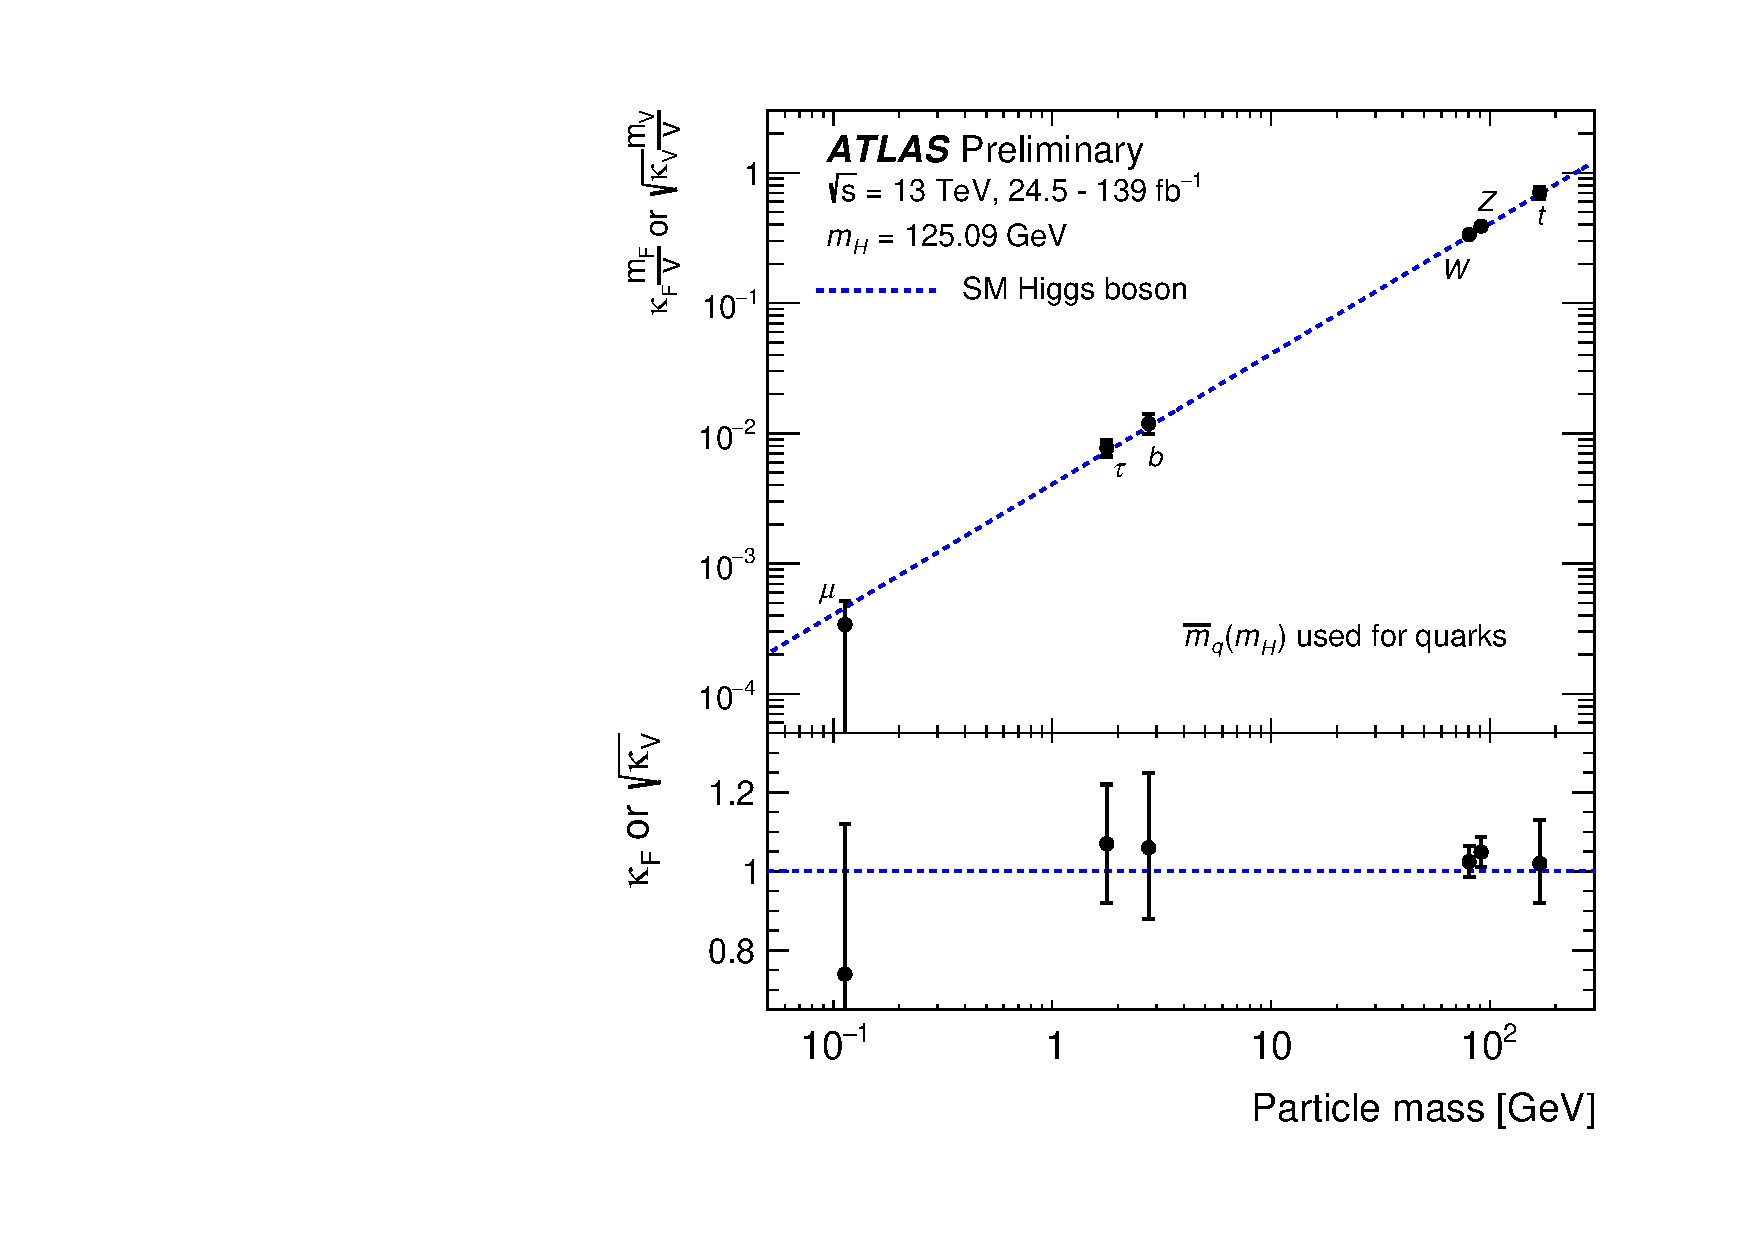
\includegraphics[width=0.85\textwidth]{figures/theory/yukawa}
  \caption[Yukawa couplings]{The reduced coupling-strength modifiers
  for fermions ($t$, $b$, $\tau$, $\mu$) and bosons ($W$, $Z$) as
  a function of their masses. The black error bars represent
  68\% CL intervals for the measured parameters. The SM
  Higgs boson prediction is shown as a blue dashed line. The
  bottom panel shows the ratio of the measured result and their
  SM values. Measurement results are taken from \cite{Aad:2019mbh}
  and \cite{ATLAS-CONF-2019-028} and have used the data with
  luminosity between 24.5 and 139 $\ifb$.
  Updated figure from Ref. \cite{Aad:2019mbh}.}
   \label{fig:the:yukawa}
\end{figure}


\section{Higgs phenomenology at the LHC}

In July 2012 the ATLAS and CMS experiments reported an observation of a new elementary particle with a
mass of approximately 125 GeV, consistent with the properties of the SM Higgs boson
\cite{Aad:2012tfa, Chatrchyan:2012xdj}. The mass of the new boson was later measured
jointly by the two experiments to be $125.09 \pm 0.21 (\text{stat.}) \pm 0.11 (\text{syst.})~\GeV$
\cite{Aad:2015zhl}. Further studies of spin, parity, and production
and decay rates in both experiments have found no evidence of deviation from the SM
Higgs boson \cite{Aad:2015mxa, PhysRevD.92.012004, Khachatryan:2016vau, Aad:2019mbh}.

The four main production modes of the Higgs boson at the proton-proton ($pp$) collisions
at the Large Hadron Collider (LHC) are the gluon-gluon fusion ($\ggf$), vector boson fusion
(\vbf), associated production with a vector boson (\vh), and the associated production with
a $\ttbar$ pair ($\tth$), all shown in Figure \ref{fig:the:prod}.

\begin{figure}[h]
  \centering
  \begin{subfigure}[b]{0.5\textwidth}
    \centering
    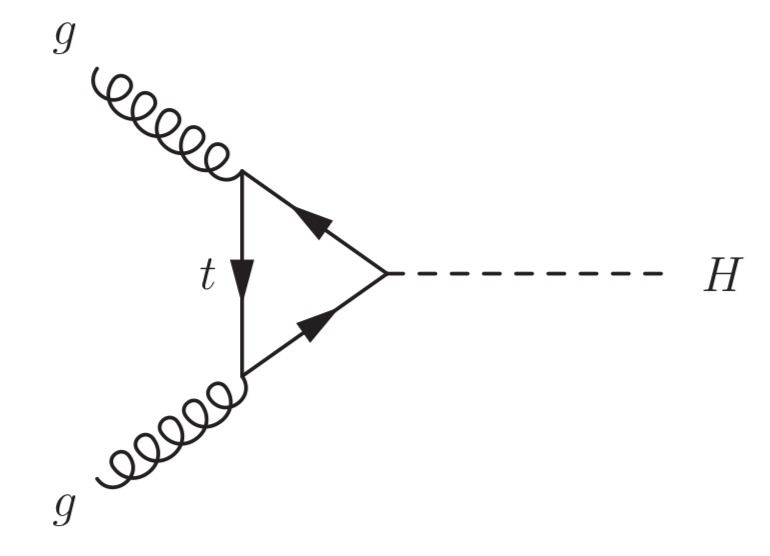
\includegraphics[width=0.8\textwidth]{figures/theory/ggF}
    \caption{$\ggf$}
  \end{subfigure}%
  \begin{subfigure}[b]{0.5\textwidth}
    \centering
    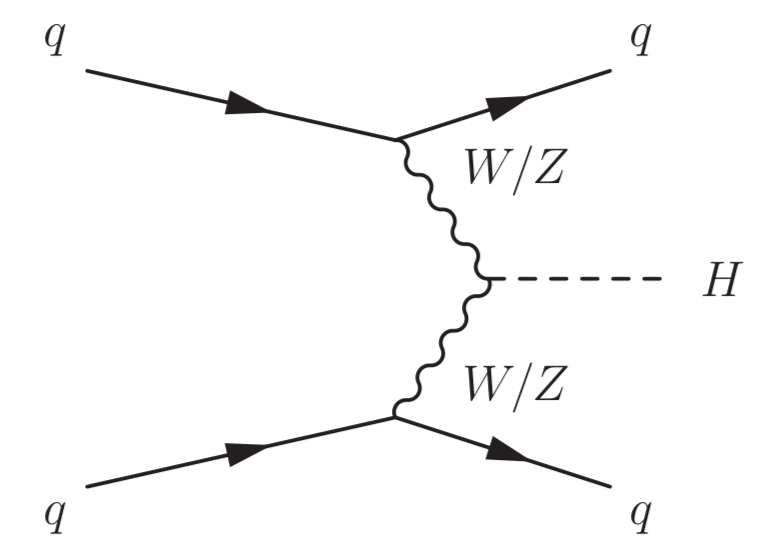
\includegraphics[width=0.8\textwidth]{figures/theory/VBF}
    \caption{$\vbf$}
  \end{subfigure}
  \begin{subfigure}[b]{0.5\textwidth}
    \centering
    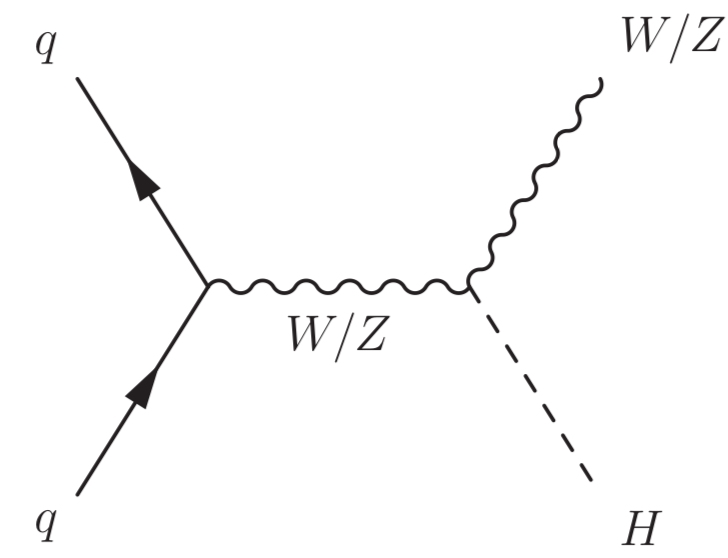
\includegraphics[width=0.8\textwidth]{figures/theory/VH}
    \caption{$\vh$}
  \end{subfigure}%
  \begin{subfigure}[b]{0.5\textwidth}
    \centering
    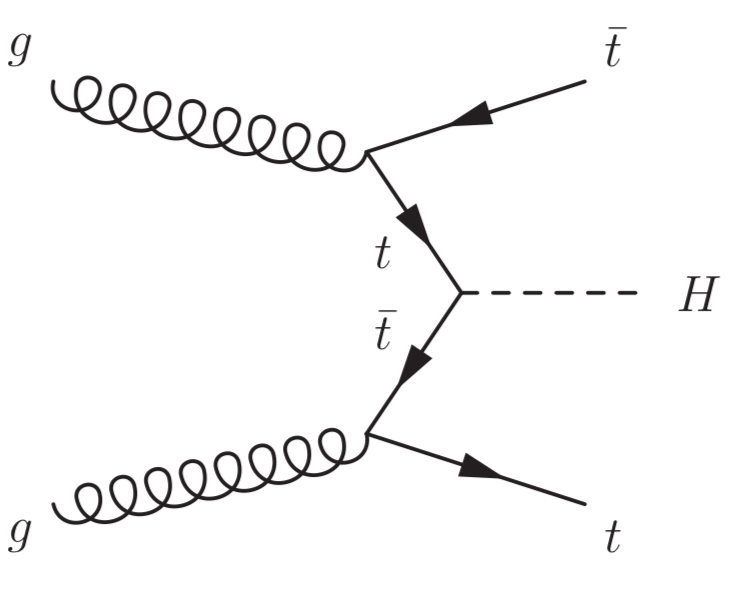
\includegraphics[width=0.8\textwidth]{figures/theory/ttH}
    \caption{$\tth$}
  \end{subfigure}
  \caption[Four main Higgs boson production modes at the LHC]
  {The Feynman diagrams for the four main Higgs boson production modes at the LHC.
  $\ggf$ process is shown in the top left, $\vbf$ in the top right, $\vh$ in bottom left, and
  $\tth$ in the bottom right subfigure.}
   \label{fig:the:prod}
\end{figure}

The majority of the Higgs bosons at the LHC are produced via the $\ggf$ production mode,
followed by $\vbf$, $\vh$, and $\tth$ production. Another two production modes are $\bbh$
and $\tH$, but they are more difficult to tag experimentally. The cross-sections and
relative fractions depend on the centre-of-mass energy as shown in Figure \ref{fig:the:prod}.
At 13 \TeV, the production cross-section for the $\ggf$ production mode is
$\sigma_{\ggf} = 48.58~\pb
~^{+4.56\%}_{-6.72\%}~(\text{theory})
\pm 3.20\%~(\text{PDF}+\alpha_S)$,
where $\alpha_S$ refers to the strong
coupling constant \cite{deFlorian:2016spz}. The total cross-section for the $\vbf$ production mode is
$\sigma_{\vbf} = 3781.7~\fb
~^{+0.43\%}_{-0.33\%}~(\text{scale})
\pm 2.1\%~(\text{PDF}+\alpha_S) $ \cite{deFlorian:2016spz}.

\begin{figure}[h]
  \centering
  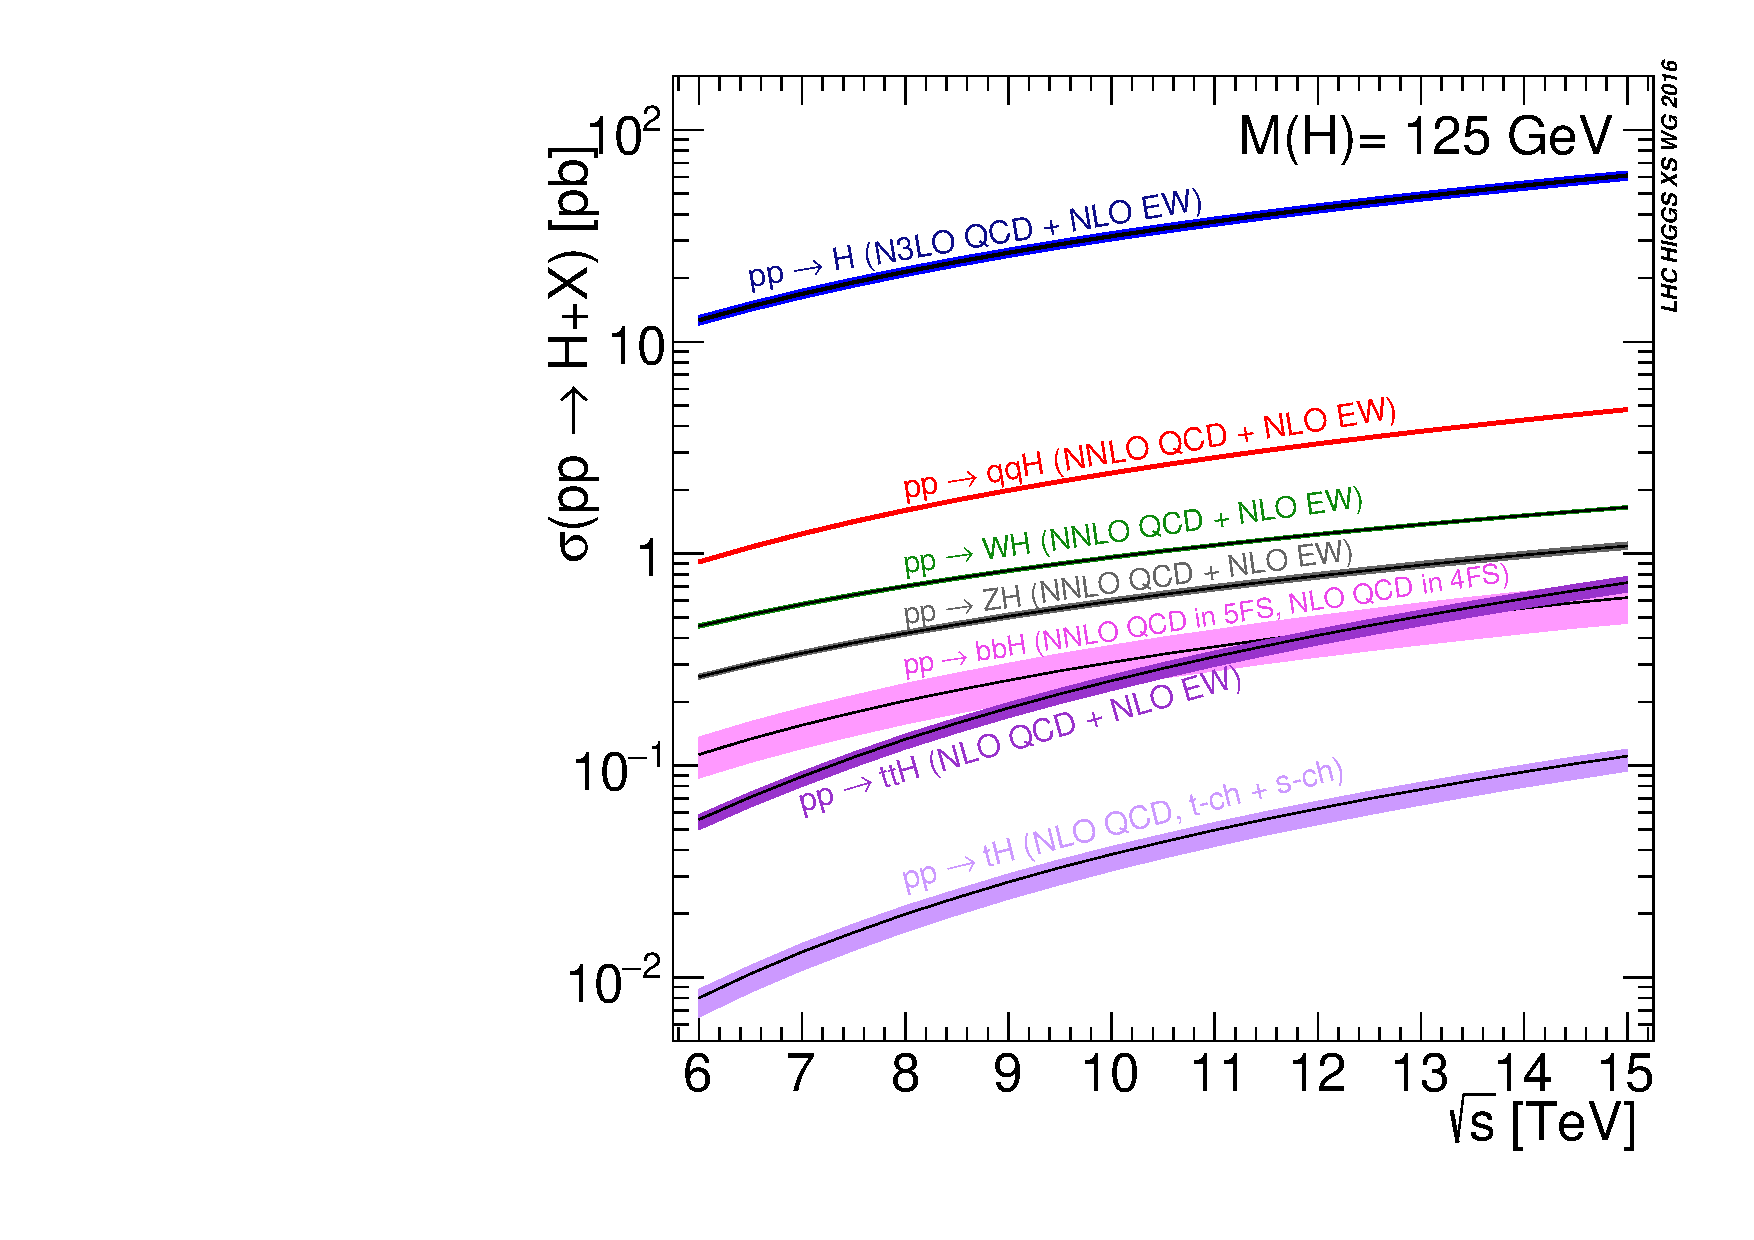
\includegraphics[width=0.8\textwidth]{figures/theory/HiggsProduction}
  \caption[Higgs boson production cross-sections at the LHC]{The Higgs boson production
  cross-sections at the LHC as a function of centre-of-mass energy, for a Higgs boson
  of mass $m_H = 125$ \GeV. $\ggf$ production cross-section is shown in blue
  ($pp \rightarrow H$), $\vbf$ in red ($pp \rightarrow qqH$), and $\tth$ in purple
  ($pp \rightarrow ttH$), while $\vh$ is shown separately for the $W$ and $Z$ bosons
  in green and gray, respectively. Reproduced from Ref. \cite{deFlorian:2016spz}.}
   \label{fig:the:prod}
\end{figure}

The Higgs boson is an unstable particle and can decay in a variety of ways. As noted,
the strength of the interaction with bosons and fermions is proportional to the mass,
meaning that the Higgs boson preferentially decays to the heavier particles, if the decays
are kinematically allowed. Figure \ref{fig:the:decay} shows the Higgs boson branching
ratios, defined as the fractions of the rate of a particular decay to the total
rate of decay. For the SM Higgs boson with $m_H = 125~\GeV$, the predicted branching ratio
to muon pairs is $2.176 \times 10^{-4}
\pm 1.23\%~(\text{theory})
\pm 0.99\%~(\text{quark mass})
\pm 0.64\%~(\alpha_S)$ \cite{deFlorian:2016spz}. 

\begin{figure}[h]
  \centering
  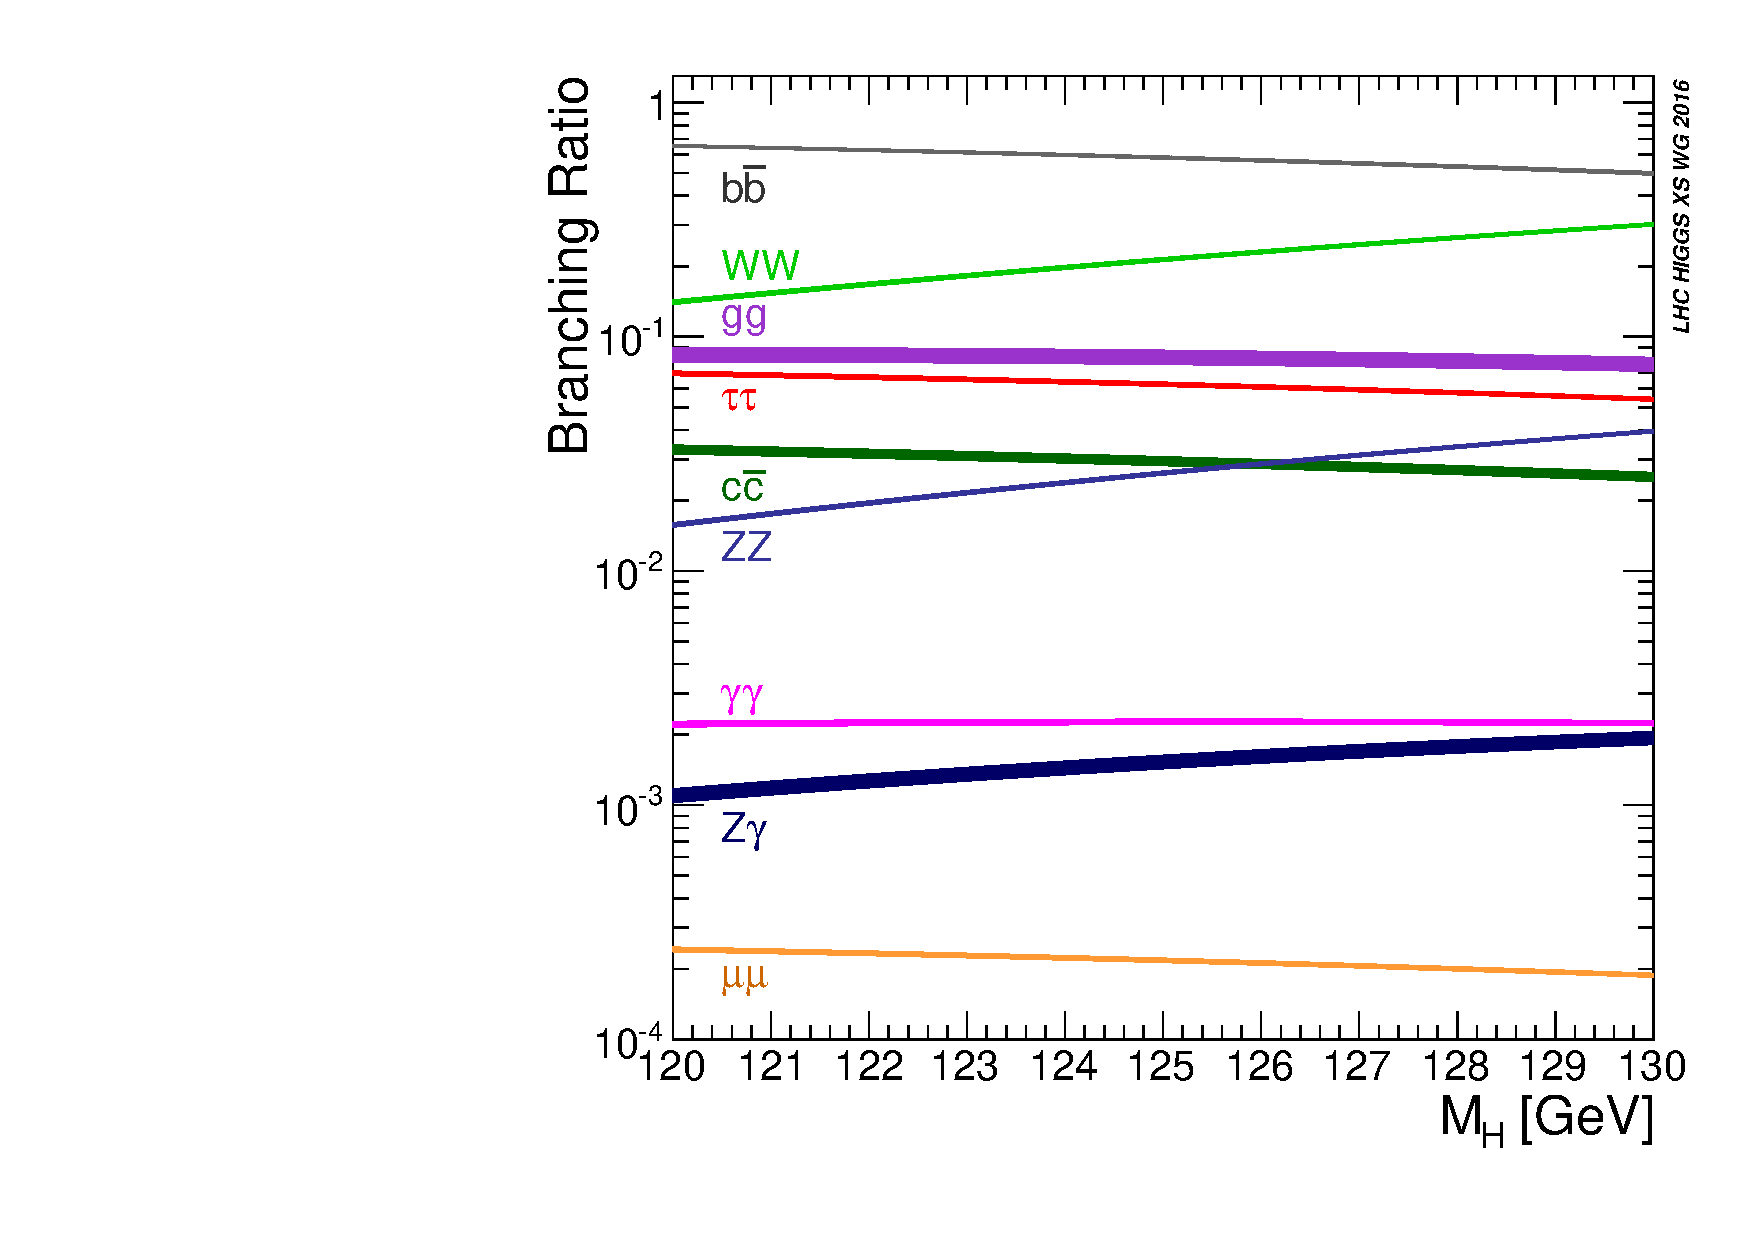
\includegraphics[width=0.8\textwidth]{figures/theory/HiggsDecay}
  \caption[Higgs boson branching ratios]{The Higgs boson branching ratios as a function
  of the Higgs boson mass. The branching ratio to muon pairs is shown in orange.
  Reproduced from Ref. \cite{deFlorian:2016spz}.}
   \label{fig:the:decay}
\end{figure}

\section{Shortcomings}

The success
of the predictive power of the Standard Model is unparalleled in the history of science.
It has been tested to unprecedented levels of numerical precision and even predicted new
fundamental particles before any experimental evidence for their existence. However,
despite its successes, the SM has numerous shortcomings.

Experimentally, while it makes exceptionally
precise predictions on a vast number of the results of measurements over many orders
of magnitude, there are a few observations that it is unable to explain at all.
Cosmological observations have firmly established the existence of dark matter via its
gravitational interactions \cite{Zwicky2008, rotation}, measurements of the
cosmological parameters from the CMB power spectrum \cite{Ade:2015}, and the
distribution of the baryonic and total mass densities in the Bullet cluster
\cite{Clowe:2006}. Similarly, there is evidence for dark energy
from the Type 1a supernovae brightness-redshift relationship
\cite{Knop:2003iy} and the cosmic microwave background spectrum \cite{Ade:2015}. Neither dark matter nor
dark energy can be explained by the SM. Similarly, the SM is unable to explain the
matter-antimatter asymmetry in the universe \cite{sarkar2007particle}.

From the theoretical perspective it is unsatisfactory that there is no quantum field description of gravity
in the SM. Additionally, the bare mass of the Higgs boson is considered to be
unnaturally close to its quantum corrections \cite{Schwartz:2013pla}.

All of these shortcomings suggest that the SM is not a complete description of Nature.
Two complementary experimental strategies to search for physics beyond the SM are
employed at the LHC. The first approach directly searches
for yet unobserved phenomena that would reveal new particles. The second approach tests
the predictions of the SM in search for a discrepancy which would signal the direction
in which direct searches should be made. While the results of direct approaches are
more easily interpretable, the advantage of indirect approaches is that they can probe
particles kinematically inaccessible at the LHC. This thesis utilises the second
approach via the search for the decay of the Higgs boson to a muon pair. Any
statistically significant discrepancy between the measured and theoretically predicted
values would hint at the existence of new physics.

